\immediate\write18{tex tqft.dtx}
\immediate\write18{tex tqft-pic.dtx}
\documentclass{article}
\usepackage{tikz}
\usetikzlibrary{shapes.geometric,tqft}
%\usepackage{tqft}

\pgfkeys{
  /do stuff/.code={
    \message{doing stuff}
  },
  /stuff/.is family,
  /stuff/.style={/do stuff},
  /stuff/.cd,
  do stuff/.code={
    \message{doing more stuff}
  },
  /stuff,
  do stuff
}

\makeatletter

\ifcsname pgfk@/handlers/.pic/.@cmd\endcsname
\message{hello}
\else
\message{goodbye}
\fi

\pgfdeclareshape{test shape}{
  \savedanchor{\centerpoint}{
    \pgfmoveto{\pgfqpoint{0pt}{0pt}}
    \pgfgetlastxy{\my@x}{\my@y}
\pgftransformyscale{-1}\pgftransformrotate{90}\pgftransformshift{\pgfqpoint{1cm}{1cm}}
    \pgfmoveto{\pgfqpoint{0pt}{0pt}}
    \pgfgetlastxy{\my@xa}{\my@ya}
    \pgf@x=-\my@x\relax
    \pgf@y=-\my@y\relax
    \advance\pgf@x by \my@xa\relax
    \advance\pgf@y by \my@ya\relax
%    \showthe\pgf@x
%    \showthe\pgf@y
  }
  \anchor{center}{\centerpoint}
\backgroundpath{
\pgftransformyscale{-1}\pgftransformrotate{90}
  \pgf@process{\pgfqpoint{0pt}{0pt}}
  \pgfpathmoveto{\pgfqpoint{0pt}{0pt}}
  \pgfpathlineto{\pgfqpoint{1cm}{0pt}}
    \pgfpathellipse{\pgfqpoint{0pt}{0pt}}{\pgfqpoint{1cm}{0pt}}{\pgfqpoint{0pt}{2cm}}
  }
}

\def\tqftpos#1#2{%
  \tqft@process{#1}{#2}%
  \showthe\pgf@x
  \showthe\pgf@y
}


%% %\tikzset{tqft/flow = east}
%% \pgfkeys{/pgf/tqft/genus/.initial = 0}
%% \pgfkeys{/pgf/tqft/anchor/.initial = none}
%% \tikzset{show name/.code={\show\tikz@fig@name}}
%% \def\tqftval#1{\pgfkeysvalueof{/pgf/tqft/#1}}

%% \tikzset{
%%   cobordism/.pic={
%% % Defining the cobordism paths
%%       \gdef\tqft@fullpath{}%
%%       \gdef\tqft@bpath{}%
%%       \gdef\tqft@gclip{}%
%%       \gdef\tqft@gpath{}%
%%       \let\tqft@clist\pgfutil@gobble%
%%       \ifnum\tqftval{incoming boundary components}>0\relax
%%       \xdef\tqft@fullpath{%
%%         \tqft@fullpath
%%         (-\tqftval{circle width},0) arc[start %% angle=\pgf@tqft@upper180, end angle=0, x radius=\tqftval{circle %% width}, y radius=\tqftval{circle depth}]
%%       }%
%%       \xdef\tqft@bpath{\tqft@bpath (-\tqftval{circle width},0) %% (\tqftval{circle width},0)}%
%%       \ifnum\tqftval{incoming boundary components}>1\relax
%%       \foreach[
%%         evaluate=\k as \xpos using (\k-1)*\tqftval{boundary %% separation} -\tqftval{circle width},
%%         evaluate=\k as \cpos using (\k-1.5)*\tqftval{boundary %% separation},
%%         evaluate=\k as \kmo using int(\k-1)
%%       ] \k in {2,...,\tqftval{incoming boundary components}} {
%%         \xdef\tqft@fullpath{%
%%           \tqft@fullpath
%%            .. controls +(0,-\tqftval{cobordism height}/3) and %% +(0,-\tqftval{cobordism height}/3) ..  (\xpos pt,0) arc[start %% angle=\pgf@tqft@upper180, end angle=0, x radius=\tqftval{circle %% width}, y radius=\tqftval{circle depth}]
%%       }%
%%         \xdef\tqft@bpath{%
%%           \tqft@bpath
%%            .. controls +(0,-\tqftval{cobordism height}/3) and %% +(0,-\tqftval{cobordism height}/3) .. (\xpos pt,0) %% ++(2*\tqftval{circle width},0)
%%       }%
%%       \xdef\tqft@clist{%
%%         \tqft@clist,-between incoming \kmo\space and \k/{(\cpos %% pt,-\tqftval{cobordism height}/4)}
%%       }%
%%       }%
%%       \fi
%%       \ifnum\tqftval{outgoing boundary components}>0\relax
%%         \pgfmathsetmacro\xppos{(\tqftval{outgoing boundary components} %% -1+\tqftval{offset}) * \tqftval{boundary separation} +\tqftval{circle %% width}}
%%       \xdef\tqft@fullpath{%
%%         \tqft@fullpath
%%         .. controls +(0,-\tqftval{cobordism height}/3) and %% +(0,\tqftval{cobordism height}/3) .. (\xppos pt, -\tqftval{cobordism %% height})
%%       }%
%%       \xdef\tqft@bpath{%
%%         \tqft@bpath
%%         .. controls +(0,-\tqftval{cobordism height}/3) and %% +(0,\tqftval{cobordism height}/3) .. (\xppos pt, -\tqftval{cobordism %% height})
%%       }%
%%       \pgfmathsetmacro\xppos{(\xppos + (\tqftval{incoming boundary %% components} -1) * \tqftval{boundary separation} +\tqftval{circle %% width})/2}%
%%       \xdef\tqft@clist{%
%%         \tqft@clist,-between last incoming and last outgoing/{(\xppos %% pt,-\tqftval{cobordism height}/2)}
%%       }%
%%       \else
%%       \pgfmathsetmacro\tqftht{\tqftval{incoming boundary %% components}/(\tqftval{incoming boundary components}+1)}
%%       \xdef\tqft@fullpath{%
%%         \tqft@fullpath
%%         .. controls +(0,-\tqftht*\tqftval{cobordism height}) and %% +(0,-\tqftht*\tqftval{cobordism height}) .. (-\tqftval{circle %% width},0)
%%       }%
%%       \xdef\tqft@bpath{%
%%         \tqft@bpath
%%         .. controls +(0,-\tqftht*\tqftval{cobordism height}) and %% +(0,-\tqftht*\tqftval{cobordism height}) .. (-\tqftval{circle %% width},0)
%%       }%
%%       \pgfmathsetmacro\xppos{(\tqftval{incoming boundary components} %% -1) * \tqftval{boundary separation}/2}%
%%       \xdef\tqft@clist{%
%%         \tqft@clist,-between first incoming and last incoming/{(\xppos %% pt,-\tqftht*\tqftval{cobordism height}*3/4)}
%%       }%
%%       \fi
%%       \else
%%       \ifnum\tqftval{outgoing boundary components}>0\relax
%%         \pgfmathsetmacro\xppos{(\tqftval{outgoing boundary components} %% -1+\tqftval{offset}) * \tqftval{boundary separation} +\tqftval{circle %% width}}
%%       \xdef\tqft@fullpath{%
%%         \tqft@fullpath
%%         (\xppos pt, -\tqftval{cobordism height})
%%       }%
%%       \xdef\tqft@bpath{%
%%         \tqft@bpath
%%         (\xppos pt, -\tqftval{cobordism height})
%%       }%
%%       \fi
%%       \fi
%% %
%%       \ifnum\tqftval{outgoing boundary components}>0\relax
%%       \pgfmathsetmacro\xppos{(\tqftval{outgoing boundary components} %% -1+\tqftval{offset}) * \tqftval{boundary separation} -\tqftval{circle %% width}}%
%%       \xdef\tqft@fullpath{%
%%         \tqft@fullpath
%%         arc[end angle=\pgf@tqft@upper180, start angle=0, x %% radius=\tqftval{circle width}, y radius=\tqftval{circle depth}]
%%       }%
%%       \xdef\tqft@bpath{\tqft@bpath (\xppos pt,-\tqftval{cobordism %% height})}%
%%       \ifnum\tqftval{outgoing boundary components}>1\relax
%%       \foreach[
%%         evaluate=\k as \xpos using (\tqftval{outgoing boundary %% components} - \k + \tqftval{offset})*\tqftval{boundary separation} + %% \tqftval{circle width},
%%         evaluate=\k as \cpos using (\tqftval{outgoing boundary %% components} - \k + .5 + \tqftval{offset})*\tqftval{boundary %% separation},
%%         evaluate=\k as \nk using int(\tqftval{outgoing boundary %% components} - \k + 1),
%%         evaluate=\k as \nkpo using int(\tqftval{outgoing boundary %% components} - \k + 2),
%%       ] \k in {2,...,\tqftval{outgoing boundary components}} {
%%         \xdef\tqft@fullpath{%
%%           \tqft@fullpath
%%            .. controls +(0,\tqftval{cobordism height}/3) and %% +(0,\tqftval{cobordism height}/3) ..  (\xpos pt,-\tqftval{cobordism %% height}) arc[end angle=\pgf@tqft@upper180, start angle=0, x %% radius=\tqftval{circle width}, y radius=\tqftval{circle depth}]
%%       }%
%%         \xdef\tqft@bpath{%
%%           \tqft@bpath
%%            .. controls +(0,\tqftval{cobordism height}/3) and %% +(0,\tqftval{cobordism height}/3) ..  (\xpos pt,-\tqftval{cobordism %% height}) ++(-2*\tqftval{circle width},0)
%%       }%
%%       \xdef\tqft@clist{%
%%         \tqft@clist,-between outgoing \nk\space and \nkpo/{(\cpos %% pt,-3*\tqftval{cobordism height}/4)}
%%       }%
%%       }%
%%       \fi
%%       \ifnum\tqftval{incoming boundary components}>0\relax
%%       \xdef\tqft@fullpath{%
%%         \tqft@fullpath
%%         .. controls +(0,\tqftval{cobordism height}/3) and %% +(0,-\tqftval{cobordism height}/3) .. (-\tqftval{circle width},0)
%%       }%
%%       \xdef\tqft@bpath{%
%%         \tqft@bpath
%%         .. controls +(0,\tqftval{cobordism height}/3) and %% +(0,-\tqftval{cobordism height}/3) .. (-\tqftval{circle width},0)
%%       }%
%%       \xdef\tqft@clist{%
%%         \tqft@clist,-between first incoming and first %% outgoing/{(\tqftval{offset}*\tqftval{boundary %% separation}/2-\tqftval{circle width},-\tqftval{cobordism height}/2)}
%%       }%
%%       \else
%%       \pgfmathsetmacro\xppos{(\tqftval{outgoing boundary components} %% -1+\tqftval{offset}) * \tqftval{boundary separation} +\tqftval{circle %% width}}%
%%       \pgfmathsetmacro\tqftht{\tqftval{outgoing boundary %% components}/(\tqftval{outgoing boundary components}+1)}
%%       \xdef\tqft@fullpath{%
%%         \tqft@fullpath
%%         .. controls +(0,\tqftht*\tqftval{cobordism height}) and %% +(0,\tqftht*\tqftval{cobordism height}) .. (\xppos %% pt,-\tqftval{cobordism height})
%%       }%
%%       \xdef\tqft@bpath{%
%%         \tqft@bpath
%%         .. controls +(0,\tqftht*\tqftval{cobordism height}) and %% +(0,\tqftht*\tqftval{cobordism height}) .. (\xppos %% pt,-\tqftval{cobordism height})
%%       }%
%%       \fi
%%       \fi
%%       \pgfmathsetmacro\xpos{%
%%         (
%%         \tqftval{outgoing boundary components} > 0 ? 
%%         (
%%         \tqftval{incoming boundary components} > 0 ?
%%         min(0,\tqftval{offset}) : \tqftval{offset}
%%         ) : 0
%%         )
%%         *\tqftval{boundary separation} - 2*\tqftval{circle width}}%
%%       \xdef\tqft@gclip{(\xpos pt,2*\tqftval{circle depth}) rectangle %% }%
%%       \pgfmathsetmacro\xpos{%
%%         ((
%%         \tqftval{outgoing boundary components} > 0 ? 
%%         (
%%         \tqftval{incoming boundary components} > 0 ?
%%         max(\tqftval{incoming boundary components},\tqftval{outgoing %% boundary components} + \tqftval{offset}) : \tqftval{outgoing boundary %% components} + \tqftval{offset}
%%         ) : \tqftval{incoming boundary components}
%%         )-1)
%%         *\tqftval{boundary separation} + 2*\tqftval{circle width}}%
%%       \xdef\tqft@gclip{\tqft@gclip (\xpos pt,-\tqftval{cobordism %% height} - 2*\tqftval{circle depth})}%
%% % Figure out the genus paths
%%       \ifnum\tqftval{genus}>0\relax
%% % Work out the left-hand edge of the cobordism
%%       \pgfmathsetmacro\xpos{%
%%         (
%%         \tqftval{outgoing boundary components} > 0 ? 
%%         (
%%         \tqftval{incoming boundary components} > 0 ?
%%         \tqftval{offset}/2 : \tqftval{offset}
%%         ) : 0
%%         )
%%         *\tqftval{boundary separation} - \tqftval{circle width}}%
%% % Work out the height that the holes should be punched at
%%       \pgfmathsetmacro\ypos{%
%%         (
%%         \tqftval{outgoing boundary components} > 0 ? 
%%         (
%%         \tqftval{incoming boundary components} > 0 ?
%%         -\tqftval{cobordism height}/2 : -1 + \tqftval{cobordism %% height}/3
%%         ) : - \tqftval{cobordism height}/3
%%         )}%
%% % Start our paths at these points
%%       \xdef\tqft@gclip{%
%%         \tqft@gclip
%%         (\xpos pt,\ypos pt)
%%       }%
%%       \xdef\tqft@gpath{%
%%         \tqft@gpath
%%         (\xpos pt,\ypos pt)
%%       }%
%% % Now work out the width of the cobordism, in units of circle %% half-widths.
%%       \pgfmathsetmacro\gsize{%
%%         ((
%%         \tqftval{outgoing boundary components} > 0 ? 
%%         (
%%         \tqftval{incoming boundary components} > 0 ?
%%         max(\tqftval{incoming boundary components},\tqftval{outgoing %% boundary components} + \tqftval{offset}) : \tqftval{outgoing boundary %% components} + \tqftval{offset}
%%         ) : \tqftval{incoming boundary components}
%%         )-1)
%%         *\tqftval{boundary separation}/\tqftval{circle width} + 2}%
%% % Each hole should take up three half-widths, but we want a little %% extra on the edges so the total number of half-widths we want is %% 3*genus + 1
%% %
%% % Do we need to scale down the holes (we never scale up)?
%% % If so, this holds the overall scale factor which we convert to x and %% y scales in points
%%       \pgfmathsetmacro\gscale{min(1,\gsize/(3*\tqftval{genus}+1))}%
%%       \pgfmathsetmacro\gyscale{\tqftval{circle depth}*\gscale*.707}%
%%       \pgfmathsetmacro\gxscale{\tqftval{circle width}*\gscale}%
%% % Each hole should take up 2 half widths, modulo scaling, so the total %% width used by the holes is 2*genus*gscale leaving gsize - %% 2*genus*gscale left for the gaps which is divided in to genus + 1 %% lots.
%%       \pgfmathsetmacro\gsep{((\gsize - %% 2*\tqftval{genus}*\gscale)/(\tqftval{genus} + 1)*\tqftval{circle %% width}}%
%%       \xdef\tqft@gclip{%
%%         \tqft@gclip
%%         ++(\gsep/2 pt,0)
%%       }%
%%       \xdef\tqft@gpath{%
%%         \tqft@gpath
%%         ++(\gsep/2 pt,0)
%%       }%
%%       \pgfmathsetmacro\xpos{1 - 1/sqrt(2)}%
%%       \pgfmathsetmacro\sqrtwo{sqrt(2)}%
%%       \foreach \k in {1,...,\tqftval{genus}} {
%%         \xdef\tqft@gclip{%
%%           \tqft@gclip
%%           ++(\gsep/2 pt + \xpos*\gxscale pt,0)
%%           .. controls +(\gxscale*\sqrtwo/3 pt,4/3*\gyscale pt) and %% +(-\gxscale*\sqrtwo/3 pt,4/3*\gyscale pt)
%%           .. ++(\sqrtwo*\gxscale pt,0)
%%           .. controls +(-\gxscale*\sqrtwo/3 pt,-4/3*\gyscale pt) and %% +(\gxscale*\sqrtwo/3 pt,-4/3*\gyscale pt)
%%           .. ++(-\sqrtwo*\gxscale pt,0)
%%           ++(2*\gxscale pt -\xpos*\gxscale pt + \gsep/2 pt,0)
%%         }
%%         \xdef\tqft@gpath{%
%%           \tqft@gpath
%%           ++(\gsep/2 pt,\pgf@tqft@upper\gyscale pt)
%%           +(\gxscale pt,\pgf@tqft@lower\gyscale pt) %% coordinate[name=-hole \k]
%%           ++(0,0)
%%           .. controls +(\gxscale pt*2/3,\pgf@tqft@lower8/3*\gyscale %% pt) and +(-\gxscale pt*2/3,\pgf@tqft@lower8/3*\gyscale pt)
%%           .. ++(2*\gxscale pt,0)
%%           ++(0,\pgf@tqft@lower2*\gyscale pt)
%%           ++(-\xpos*\gxscale pt,\pgf@tqft@upper\gyscale pt)
%%           .. controls +(-\gxscale %% pt*\sqrtwo/3,\pgf@tqft@upper4/3*\gyscale pt) and +(\gxscale %% pt*\sqrtwo/3,\pgf@tqft@upper4/3*\gyscale pt)
%%           .. ++(-\sqrtwo*\gxscale pt,0)
%%           ++(-\xpos*\gxscale pt + 2*\gxscale pt + \gsep/2 pt,0)
%%         }
%%       }
%%       \fi
%% %
%% % Now we start to lay out the cobordism
%% %
%% % Were we given a shift?  If so, shift.
%% \gdef\tqft@shift{(0,0)}%
%% \edef\tqft@anchor{-\tqftval{anchor}}%
%% \foreach \anchor/\coord in \tqft@clist
%% {
%%   \ifx\anchor\tqft@anchor\relax
%%   \expandafter\gdef\expandafter\tqft@shift\coord
%%   \fi
%% }%
%% \tikz@scan@one@point\pgfutil@firstofone\tqft@shift\relax
%% \begin{scope}[shift={(-\pgf@x,-\pgf@y)}]
%% %
%% % Incoming boundary components, nodes
%%       \ifnum\tqftval{incoming boundary components}>0\relax
%%       \foreach[evaluate=\k as \xpos using (\k-1)*\tqftval{boundary %% separation}] \k in {1,...,\tqftval{incoming boundary components}} {
%%         \node[
%%           node contents={},
%%           ellipse,
%%           inner sep=0pt,
%%           outer sep=0pt,
%%           minimum width=2*\tqftval{circle width},
%%           minimum height=2*\tqftval{circle depth},
%%           at={(\xpos pt,0)},
%%           name=-incoming boundary \k,
%%           /pgf/tqft/every boundary component/.try,
%%           /pgf/tqft/every incoming boundary component/.try,
%%           /pgf/tqft/incoming boundary component \k/.try
%%         ];
%%       }%
%%       \fi
%% % Outgoing boundary components, nodes
%%       \ifnum\tqftval{outgoing boundary components}>0\relax
%%       \foreach[
%%         evaluate=\k as \xpos using %% (\k-1+\tqftval{offset})*\tqftval{boundary                   %% separation}
%%       ] \k in {1,...,\tqftval{outgoing boundary components}} {
%%           \node[
%%           node contents={},
%%           ellipse,
%%           inner sep=0pt,
%%           outer sep=0pt,
%%           minimum width=2*\tqftval{circle width},
%%           minimum height=2*\tqftval{circle depth},
%%           at={(\xpos pt,-\tqftval{cobordism height})},
%%           name=-outgoing boundary \k,
%%           /pgf/tqft/every boundary component/.try,
%%           /pgf/tqft/every outgoing boundary component/.try,
%%           /pgf/tqft/outgoing boundary component \k/.try
%%         ];
%%       }%
%%       \fi
%% % Incoming boundary components, lower paths
%%       \ifnum\tqftval{incoming boundary components}>0\relax
%%       \foreach[evaluate=\k as \xpos using (\k-1)*\tqftval{boundary %% separation}] \k in {1,...,\tqftval{incoming boundary components}} {
%%         \path[
%%           /pgf/tqft/every lower boundary component/.try,
%%           /pgf/tqft/every incoming lower boundary component/.try,
%%           /pgf/tqft/incoming lower boundary component \k/.try
%%         ] (\xpos pt - \tqftval{circle width},0) arc[start %% angle=\pgf@tqft@lower180,end angle=0, x radius=\tqftval{circle width}, %% y radius =\tqftval{circle depth}];
%%       }%
%%       \fi
%% % Outgoing boundary components, lower paths
%%       \ifnum\tqftval{outgoing boundary components}>0\relax
%%       \foreach[
%%         evaluate=\k as \xpos using %% (\k-1+\tqftval{offset})*\tqftval{boundary                   %% separation}
%%       ] \k in {1,...,\tqftval{outgoing boundary components}} {
%%         \path[
%%           /pgf/tqft/every lower boundary component/.try,
%%           /pgf/tqft/every outgoing lower boundary component/.try,
%%           /pgf/tqft/outgoing lower boundary component \k/.try
%%         ] (\xpos pt - \tqftval{circle width},-\tqftval{cobordism %% height}) arc[start angle=\pgf@tqft@lower180,end angle=0, x %% radius=\tqftval{circle width}, y radius =\tqftval{circle depth}];
%%         }%
%%       \fi
%% % Full outer path, clipped against genus
%%       \begin{scope}
%%       \path[clip] \tqft@gclip;
%%       \path[
%%         /pgf/tqft/cobordism/.try
%%       ] \tqft@fullpath;
%%       \end{scope}
%%       \path[
%%         /pgf/tqft/cobordism/.try,
%%         fill=none,
%%         /pgf/tqft/cobordism edge/.try,
%%         /pgf/tqft/genus style/.try
%%       ] \tqft@gpath;
%% % Non-boundary path
%%       \path[
%%         /pgf/tqft/cobordism edge/.try,
%%         /pgf/tqft/cobordism outer edge/.try
%%       ] \tqft@bpath;
%% % Coordinates
%%       \ifx\tqft@clist\pgfutil@gobble
%%       \else
%%       \foreach \name/\coord in \tqft@clist {
%%         \path \coord node[coordinate,node contents={},name=\name];
%%       }
%%       \fi
%% % Incoming boundary components, upper paths
%%       \ifnum\tqftval{incoming boundary components}>0\relax
%%       \foreach[evaluate=\k as \xpos using (\k-1)*\tqftval{boundary %% separation}] \k in {1,...,\tqftval{incoming boundary components}} {
%%         \path[
%%           /pgf/tqft/every upper boundary component/.try,
%%           /pgf/tqft/every incoming upper boundary component/.try,
%%           /pgf/tqft/incoming upper boundary component \k/.try
%%         ] (\xpos pt - \tqftval{circle width},0) arc[start %% angle=\pgf@tqft@upper180,end angle=0, x radius=\tqftval{circle width}, %% y radius =\tqftval{circle depth}];
%%       }
%%       \fi
%% % Outgoing boundary components, upper paths
%%       \ifnum\tqftval{outgoing boundary components}>0\relax
%%       \foreach[
%%         evaluate=\k as \xpos using %% (\k-1+\tqftval{offset})*\tqftval{boundary                   %% separation}
%%       ] \k in {1,...,\tqftval{outgoing boundary components}} {
%%         \path[
%%           /pgf/tqft/every upper boundary component/.try,
%%           /pgf/tqft/every outgoing upper boundary component/.try,
%%           /pgf/tqft/outgoing upper boundary component \k/.try
%%         ] (\xpos pt - \tqftval{circle width},-\tqftval{cobordism %% height}) arc[start angle=\pgf@tqft@upper180,end angle=0, x %% radius=\tqftval{circle width}, y radius =\tqftval{circle depth}];
%%       }
%%       \fi
%% \end{scope}
%%   }
%% }
\makeatother
\begin{document}

\begin{tikzpicture}
\draw (0,0) --  node[name=a,coordinate] {} (2,0) .. controls +(1,0) and +(0,-1) .. node[coordinate,name=b] {} (4,1) ++(2,0) -- ++(2,0);
\draw[<-] (a) -- ++(0,1);
\draw[<-] (b) -- ++(0,1);
\foreach \coord in {{(0,0)},{(1,0)}} {
  \node (c) at \coord {};
  \draw (2,2) -- (c);
}
\end{tikzpicture}

\begin{tikzpicture}[
  tqft,
  every outgoing boundary component/.style={fill=blue!50},
  outgoing boundary component 3/.style={fill=none,draw=red},
  every incoming boundary component/.style={fill=green!50},
  every lower boundary component/.style={draw,ultra thick, dashed},
  every upper boundary component/.style={draw,purple},
  cobordism/.style={fill=red!50},
  cobordism edge/.style={draw},
  genus=3,
  genus style/.style={draw},
  view from=incoming,
  anchor=between incoming 1 and 2
]
\pic[name=a,tqft,incoming boundary components=2,outgoing boundary components=3,offset=-.5]{cobordism};
\begin{scope}[every pin edge/.style={<-}]
\foreach \anchor/\ang in {
  hole 1/-90,
  incoming boundary 2/90,
  outgoing boundary 3/-90,
  between last incoming and last outgoing/0,
  between first incoming and first outgoing/180,
  between incoming 1 and 2/90,
  between outgoing 1 and 2/-90,
  between outgoing 2 and 3/-90
} {
  \node[pin=\ang:\anchor,at=(a-\anchor)] {};
}
\draw[<-] (0,0) -- ++(0,3);
\end{scope}
\end{tikzpicture}


\begin{tikzpicture}[
  tqft,
  every outgoing boundary component/.style={fill=blue!50},
  outgoing boundary component 3/.style={fill=none,draw=red},
  every incoming boundary component/.style={fill=green!50},
  every lower boundary component/.style={draw,ultra thick, dashed},
  every upper boundary component/.style={draw,purple},
  cobordism/.style={fill=red!50},
  cobordism edge/.style={draw},
  genus=3,
  genus style/.style={draw},
  view from=incoming,
  anchor=between incoming 1 and 2
]
\pic[name=a,tqft,incoming boundary components=2,outgoing boundary components=3,offset=-.5]{cobordism};
\end{tikzpicture}

\begin{tikzpicture}[
  tqft,
  every outgoing boundary component/.style={fill=blue!50},
  outgoing boundary component 3/.style={fill=none,draw=red},
  every incoming boundary component/.style={fill=green!50},
  every lower boundary component/.style={draw,ultra thick, dashed},
  every upper boundary component/.style={draw,purple},
  cobordism/.style={draw=red!50,ultra thick},
  cobordism edge/.style={draw},
  genus=1
]
\pic[name=a,tqft,incoming boundary components=3,outgoing boundary components=0,offset=-.5]{cobordism};
\begin{scope}[every pin edge/.style={<-}]
\foreach \anchor/\ang in {
  hole 1/-90,
  incoming boundary 2/90,
  between first incoming and last incoming/-90
} {
  \node[pin=\ang:\anchor,at=(a-\anchor)] {};
}
\end{scope}
\end{tikzpicture}

\begin{tikzpicture}[
  tqft,
  every outgoing boundary component/.style={fill=blue!50},
  outgoing boundary component 3/.style={fill=none,draw=red},
  every incoming boundary component/.style={fill=green!50},
  every lower boundary component/.style={draw,ultra thick, dashed},
  every upper boundary component/.style={draw,purple},
  cobordism/.style={draw=red!50,ultra thick},
  cobordism edge/.style={draw},
]
\pic[name=a,tqft,incoming boundary components=0,outgoing boundary components=3,offset=-.5]{cobordism};
\draw (a-between first and last outgoing) -- ++(0,2);
\end{tikzpicture}

\begin{tikzpicture}[tqft/flow=south]
\node[draw,tqft,incoming boundary components=2,outgoing boundary components=3,offset=-.5] (a) {};
\end{tikzpicture}

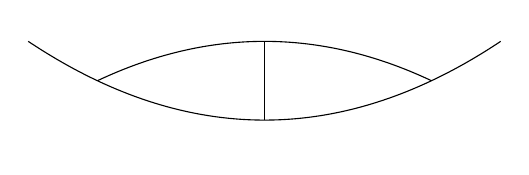
\begin{tikzpicture}
%\draw (0,0) .. controls +(2,4/3) and +(-2,4/3) .. (6,0);
\draw (0,1) .. controls +(2,-4/3) and +(-2,-4/3) .. (6,1);
\draw (3,0) -- (3,1);
\pgfmathsetmacro\xpos{(1 - 1/sqrt(2))/2}
\pgfmathsetmacro\sqrtwo{1/sqrt(2)}
\draw (6*\xpos,.5) .. controls +(2*\sqrtwo,2/3) and +(-2*\sqrtwo,2/3) .. (6 - 6*\xpos,.5);
\end{tikzpicture}


\begin{tikzpicture}[tqft/flow=east]
\node[tqft pair of pants, draw, boundary lower style={draw}] (a) {};
\node at (a.incoming boundary 1) {\(A\)};
\node at (a.outgoing boundary 1) {\(A\)};
\node at (a.outgoing boundary 2) {\(A\)};
\node at (a) {\(\beta\)};
\end{tikzpicture}


\begin{tikzpicture}[shape=tqft cobordism]
\begin{scope}[scale=2,rotate=45,tqft,flow=east,boundary lower style={draw,thick}]
\node[tqft pair of pants,draw,transform shape] {};
\end{scope}
\end{tikzpicture}
%\end{document}

\begin{tikzpicture}
\node[tqft pair of pants,draw,circle width=2cm,circle depth=1cm,cobordism height=8cm,boundary separation=2cm] {};
\end{tikzpicture}


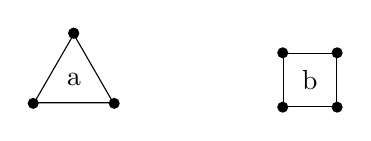
\begin{tikzpicture}
\node[regular polygon,regular polygon sides=3,draw] (a) {a};
\node[regular polygon,regular polygon sides=4,draw] (b) at (3,0) {b};
\foreach \k in {1,...,4} {
  \fill (a.corner \k) circle[radius=2pt];
}
\foreach \k in {1,...,4} {
  \fill (b.corner \k) circle[radius=2pt];
}
\end{tikzpicture}

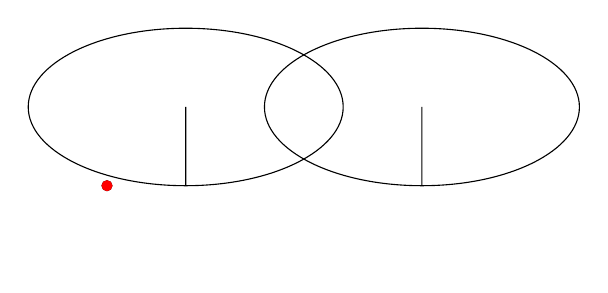
\begin{tikzpicture}
\fill (0,0) circle[radius=2pt];
\node[test shape,draw] (a) {};
\node[test shape,draw] (b) at (3,0) {};
\fill[red] (a) circle[radius=2pt];
\end{tikzpicture}

\begin{tikzpicture}[tqft/flow={east}]
\fill[orange] (0,0) circle[radius=4pt];
\node[tqft,pair of pants,draw,outer sep=1cm] (a) at (0,0) {};
\node[tqft,incoming boundary components=4,outgoing boundary components=3,offset=.5,draw] (b) at (3,0) {};
%\node[tqft,pair of pants,draw,red] (b) at (1,0) {};
%\node[tqft,pair of pants,draw,green] (c) at (0,1) {};
%\node[tqft,pair of pants,draw,blue] (d) at (-1,0) {};
%\fill (a.incoming boundary 1) circle[radius=2pt];
%\fill[red] (b.incoming boundary 1) circle[radius=2pt];
%\fill[green] (c.incoming boundary 1) circle[radius=2pt];
%\fill[blue] (d.incoming boundary 1) circle[radius=2pt];
\foreach \anchor in {
  centre,
  center,
  north,
  south,
  east,
  north west,
  south west,
  north east,
  south east,
  west%
} {
\foreach \node/\colour in {
    a/black,
    b/red%,
%    c/green,
%    d/blue%
}{
\edef\command{\noexpand\fill[\colour] (\node.\anchor) circle[radius=2pt] node {\anchor};}
\command
}
}
\end{tikzpicture}


\begin{tikzpicture}
\node[draw,outer sep=1cm] (a) {a};
\fill (a.north) circle[radius=2pt];
\end{tikzpicture}

\begin{tikzpicture}[tqft/flow={east}]
\node[tqft,boundary circle,draw] at (0,0) {};
\node[tqft,boundary circle,draw,red] at (1,0) {};
\node[tqft,boundary circle,draw,green] at (0,1) {};
\node[tqft,boundary circle,draw,blue] at (-1,0) {};
\end{tikzpicture}

\begin{tikzpicture}[every tqft/.style={cobordism style={draw,thick,red}}]
 \node[
   tqft,
   fill=orange,
   fill opacity=.5,
   boundary style={fill=purple},
   cobordism style={draw,thick,red},
   boundary lower style={draw,dashed,thick,blue},
   boundary upper style={draw,green,thick},
   incoming boundary components=4,
   outgoing boundary components=6,
   offset=-1.5,
   outer sep=1cm,
 ] (a) {};
 \fill (a incoming 2.90) circle[radius=2pt];
 \fill (a outgoing 5.270) circle[radius=2pt];
 \fill (a incoming 2.centre) circle[radius=2pt];
 \fill (a outgoing 5.centre) circle[radius=2pt];
 \fill (a incoming 4.above) circle[radius=2pt];
 \fill (a outgoing 3.below) circle[radius=2pt];
 \fill (a.after incoming boundary 1) circle[radius=2pt] node[pin=north:between 1 and 2] {};
 \fill (a.after outgoing boundary 3) circle[radius=2pt] node[pin=south:between 3 and 4] {};
 \fill (a.incoming boundary 1) circle[radius=2pt] node[pin=north:1] {};
 \fill (a.incoming boundary 2) circle[radius=2pt] node[pin=north:2] {};
 \fill (a.incoming boundary 3) circle[radius=2pt] node[pin=north:3] {};
 \fill (a.incoming boundary 4) circle[radius=2pt] node[pin=north:4] {};
 \node[pin=north:2] at (a.incoming boundary 2) {};
 \node[pin=north:3] at (a.incoming boundary 3) {};
 \node[pin=north:4] at (a.incoming boundary 4) {};
 \node[pin=south:1] at (a.outgoing boundary 1) {};
 \node[pin=south:4] at (a.outgoing boundary 4) {};
 \node[pin=south:6] at (a.outgoing boundary 6) {};
\node[pin=west:west] at (a.west) {};
\node[pin=east:east] at (a.east) {};
 \end{tikzpicture}


\begin{tikzpicture}[
  tqft,
  every outgoing boundary component/.style={fill=blue!50},
  outgoing boundary component 3/.style={fill=none,draw=red},
  every incoming boundary component/.style={fill=green!50},
  every lower boundary component/.style={draw,ultra thick, dashed},
  every upper boundary component/.style={draw,purple},
  cobordism/.style={fill=red!50},
  cobordism edge/.style={draw},
  genus=3,
  genus style/.style={draw},
  view from=incoming,
  anchor=between incoming 1 and 2
]
\pic[name=a,tqft,incoming boundary components=4,outgoing boundary components=6,offset=-1.5]{cobordism};
\end{tikzpicture}

\begin{tikzpicture}[every tqft/.style={cobordism style={draw,thick,red}}]
 \node[
   tqft,
   fill=orange,
   fill opacity=.5,
   boundary style={fill=purple},
   cobordism style={draw,thick,red},
   boundary lower style={draw,dashed,thick,blue},
   boundary upper style={draw,green,thick},
   incoming boundary components=0,
   outgoing boundary components=6,
   offset=-1.5,
   outer sep=1cm,
 ] (aa) {hello world};
% \fill (aa incoming 2.90) circle[radius=2pt];
 \fill (aa outgoing 5.270) circle[radius=2pt];
% \fill (aa incoming 2.centre) circle[radius=2pt];
 \fill (aa outgoing 5.centre) circle[radius=2pt];
% \fill (aa incoming 4.above) circle[radius=2pt];
 \fill (aa outgoing 3.below) circle[radius=2pt];
 \fill (aa.incoming boundary 1) circle[radius=2pt] node[pin=north:1] {};
 \fill (aa.incoming boundary 2) circle[radius=2pt] node[pin=north:2] {};
 \fill (aa.incoming boundary 3) circle[radius=2pt] node[pin=north:3] {};
 \fill (aa.incoming boundary 4) circle[radius=2pt] node[pin=north:4] {};
 \node[pin=north:2] at (aa.incoming boundary 2) {};
 \node[pin=north:3] at (aa.incoming boundary 3) {};
 \node[pin=north:4] at (aa.incoming boundary 4) {};
 \node[pin=south:1] at (aa.outgoing boundary 1) {};
 \node[pin=south:4] at (aa.outgoing boundary 4) {};
 \node[pin=south:6] at (aa.outgoing boundary 6) {};
\fill[cyan] (0,0) circle[radius=3pt];
\node[pin=west:west] at (aa.west) {};
\node[pin=east:east] at (aa.east) {};
\node[pin=north:north] at (aa.north) {};
 \end{tikzpicture}

\begin{tikzpicture}[tqft/flow={east},every tqft/.style={cobordism style={draw,thick,red}}]
 \node[
   tqft,
   boundary circle,
   circle width=2cm,
   circle depth=1cm,
   boundary separation=4cm,
   fill=orange,
   fill opacity=.5,
   boundary style={fill=purple},
   cobordism style={draw,thick,red},
   boundary lower style={draw,dashed,thick,blue},
   boundary upper style={draw,green,thick},
   incoming boundary components=4,
   outgoing boundary components=6,
   offset=-1.5,
 ] (a) {};
 \node[
   tqft,
   boundary circle,
   circle width=2cm,
   circle depth=1cm,
   boundary separation=4cm,
   fill=orange,
   fill opacity=.5,
   boundary style={fill=purple},
   cobordism style={draw,thick,red},
   boundary lower style={draw,dashed,thick,blue},
   boundary upper style={draw,green,thick},
   incoming boundary components=4,
   outgoing boundary components=6,
   offset=-1.5,
 ] at (5,0) (b) {hello world};
\fill[red] (b.centre) circle[radius=2pt];
 \fill[red] (b.next) circle[radius=2pt] node[pin=north:next] {};
 \fill[red] (b.prior) circle[radius=2pt] node[pin=north:prior] {};
 \fill[red] (b.above) circle[radius=2pt] node[pin=north:above] {};
 \fill[red] (b.below) circle[radius=2pt] node[pin=north:below] {};
 \fill (a.next) circle[radius=2pt] node[pin=north:next] {};
 \fill (a.prior) circle[radius=2pt] node[pin=north:prior] {};
 \fill (a.above) circle[radius=2pt] node[pin=north:above] {};
 \fill (a.below) circle[radius=2pt] node[pin=north:below] {};
 \draw (0,0) -- (90:2);
 \draw (0,0) -- (0:2);
 \draw (0,0) -- (180:2);
 \draw (0,0) -- (270:2);
\foreach \ang in {0,20,...,340} {
 \fill (a.\ang) circle[radius=2pt] node[pin=\ang:\ang] {};
 \draw (0,0) -- (\ang:2);
}
 \end{tikzpicture}

\end{document}

% Local Variables:
% tex-output-type: "pdf18"
% End: